\documentclass[twocolumn,aps,prb,citeautoscript]{revtex4-1}
\usepackage{graphicx}

\begin{document}

\title{SURF Progress Report 1:\\
Effects of superconducting lead endcaps on boundary conditions of
magnetic fields}
\author{Aritra Biswas, with Filippone Group}
\affiliation{W.K. Kellogg Radiation
Laboratory, California Institute of Technology}

%\begin{abstract}

%\end{abstract}

\maketitle

\section{Motivation}

\subsection{Group goal: the half-scale model}

The discovery of charge-parity symmetry (CP) violation 
in the decay of neutral kaons has inspired attempts to extend the
Standard Model \cite{cpv}. Measurements of the electric
dipole moments (EDM) of various particles provide important restrictions
and clues to guide new models. \cite{ill}.
The neutron electric dipole moment (nEDM) collaboration intends to
improve \cite{krl} the currently-measured limit \cite{ill}
on the neutron EDM with new experimental techniques.
Trapped ultra-cold neutrons (UCN) precess in the presence
of a constant magnetic field or a variable electric field; measuring
a change in precession correlated with the electric field
would confirm a non-zero EDM.

An important obstacle is eliminating a ``geometric phase effect''
that creates a shift in the UCN precession and results in
a false EDM reading. Since this effect is caused by field gradients,
we need to make the magnetic field as uniform as possible.
To 
tackle the engineering challenge of creating an uniform magnetic field,
we have constructed a half-scale model of the magnet that will be
used in the nEDM experiment. We are both simulating and measuring
the effects of various types of shielding ($\mu$-metal,
ferromagnetic Metglas, and superconducting lead). The ultimate goal is to
determine the optimal magnet design for the nEDM experiment.

\subsection{SURF goal: superconducting endcaps}

The current setup (fig. \ref{fig:structure})
features a cylindrical $\cos\theta$ coil \cite{coil} (referred to as the $B_0$ coil)
surrounded by concentric open-ended cylindrical shells for shielding.
In order to improve field uniformity, we investigate the effects of superconducting
lead endcaps to close the open ends of the lead shield.

Since November 2013 (when I first stared work in this group), we have designed and installed
a bottom endcap. Measurements taken afterwards suggested that a top endcap would be more
effective. As of July 2014, we have a top endcap installed on the magnet and are preparing
to cool the lead shielding to superconducting temperature.

The goal of this SURF is to help develop a reliable simulation of
this endcap, measure its effects, explain any inconsistencies, and determine how effective
this endcap style will be for the final nEDM experiment.

\begin{figure}
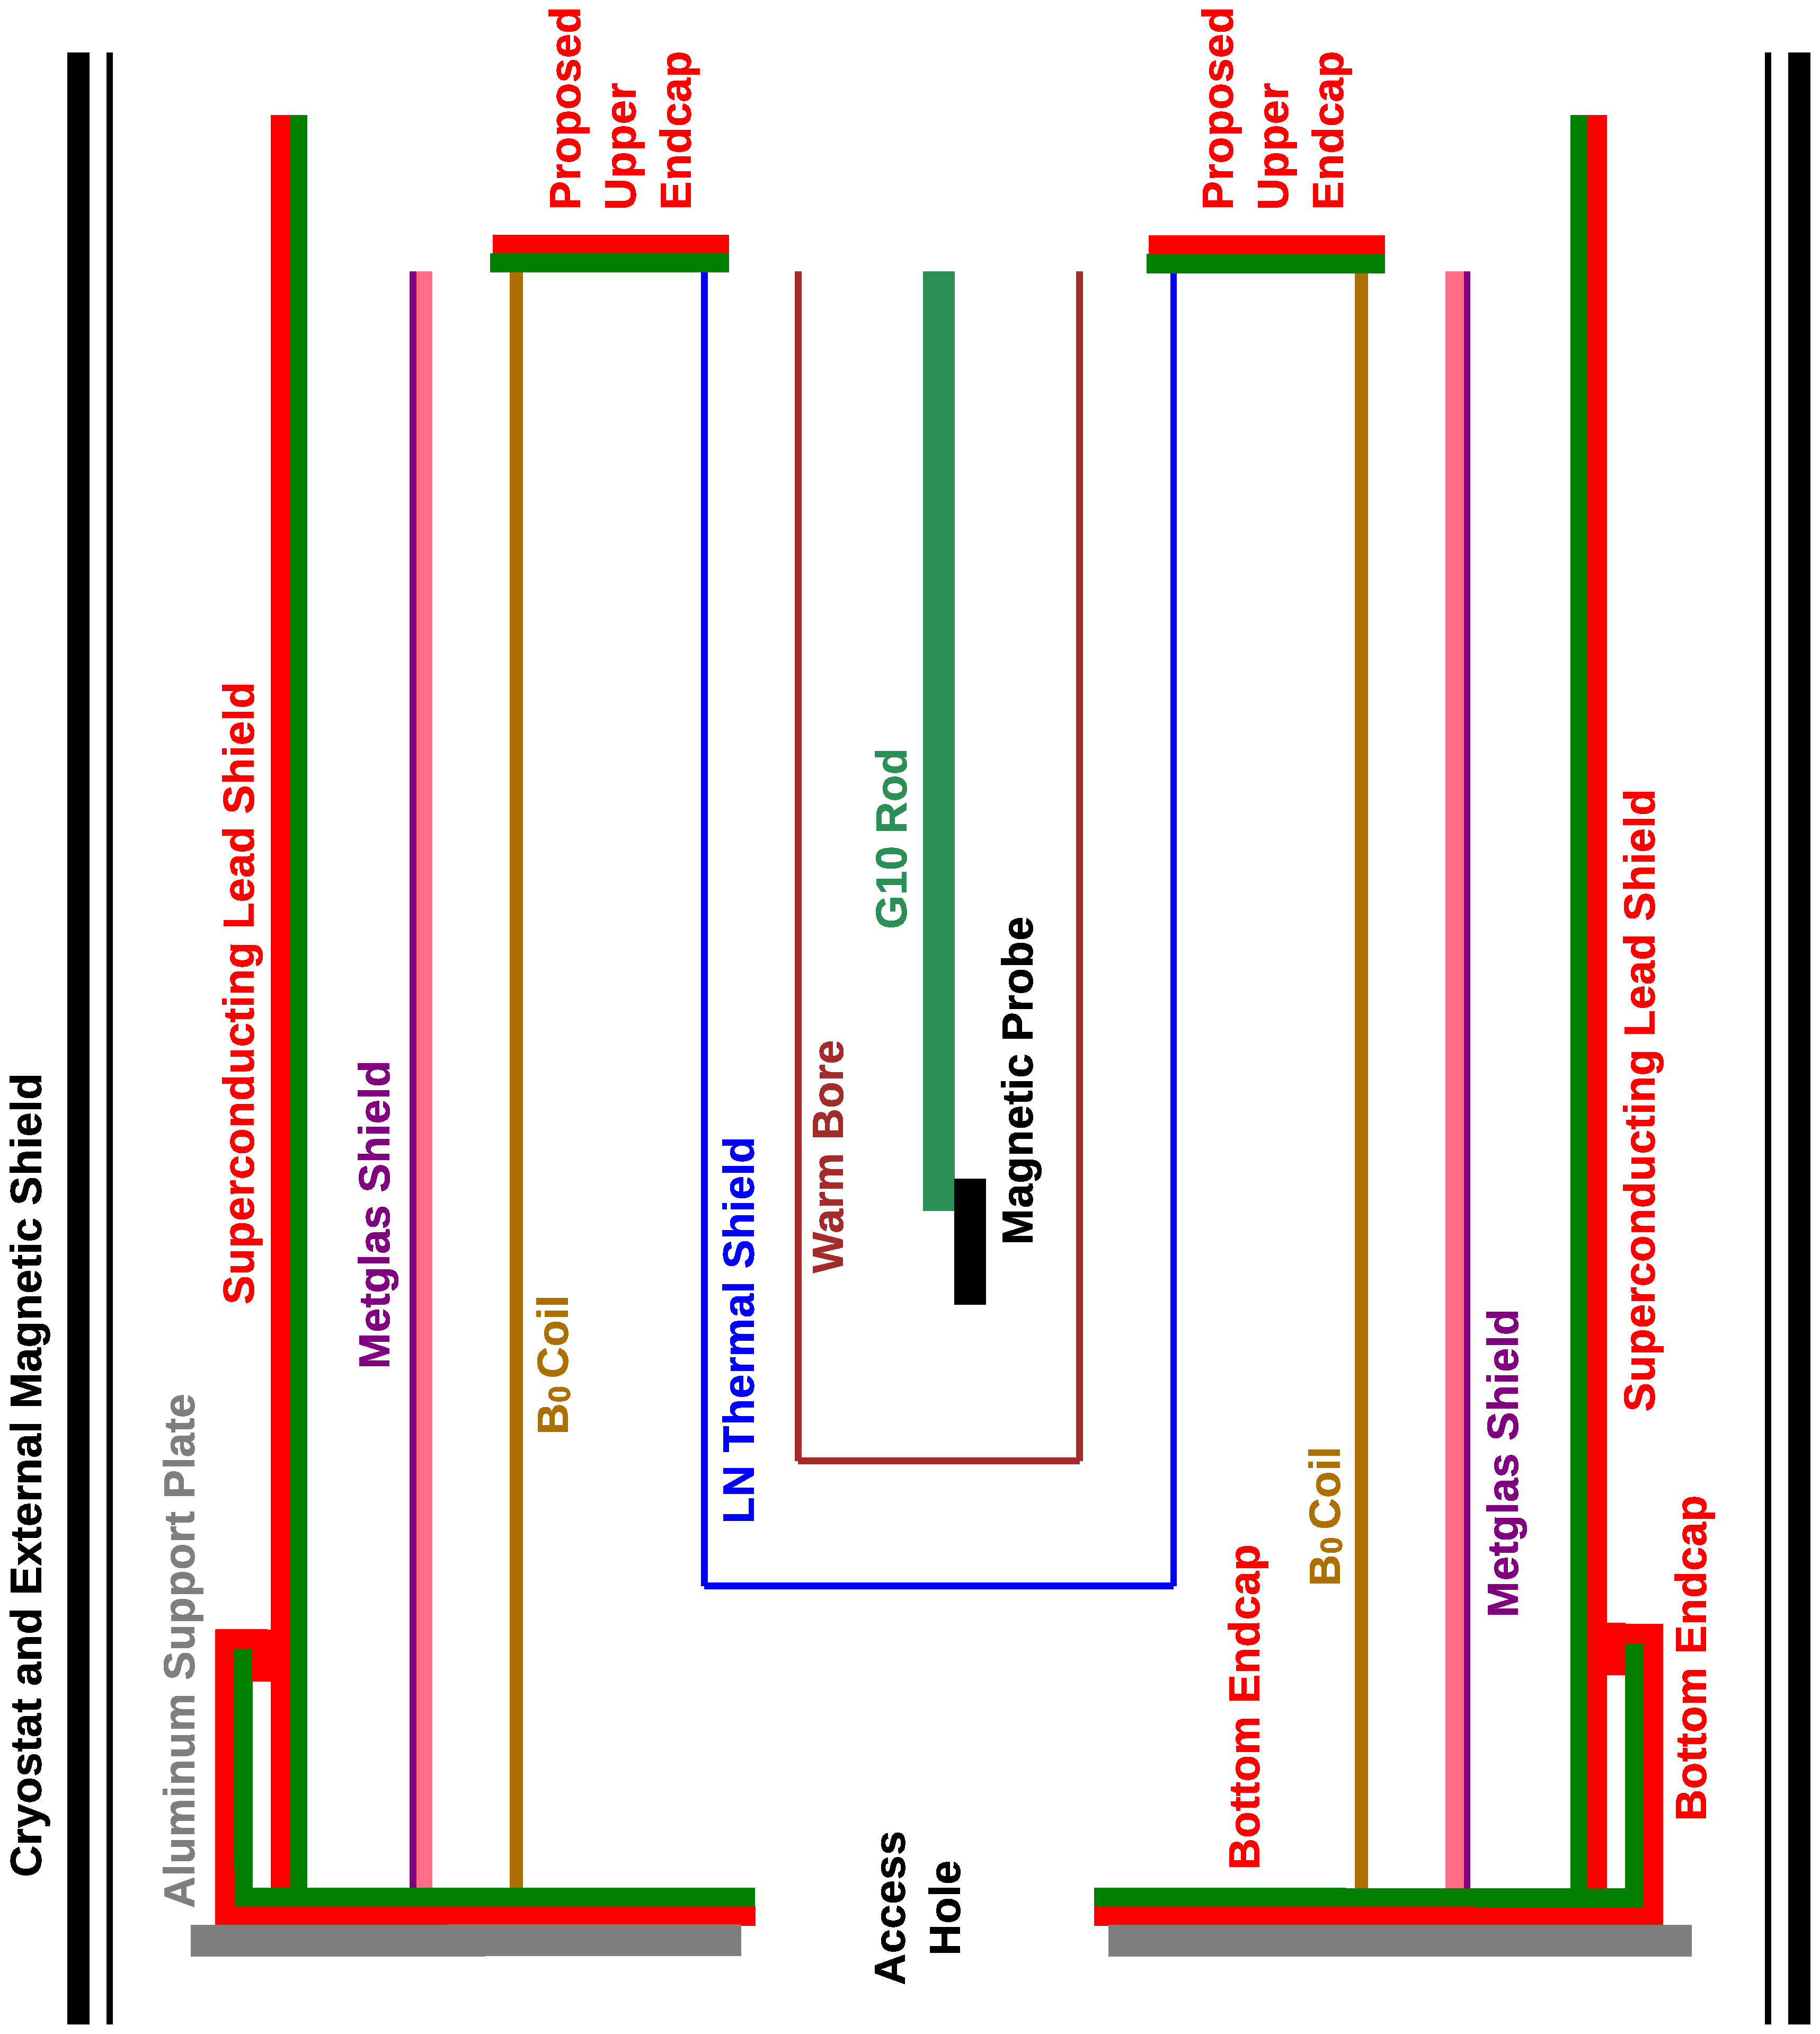
\includegraphics[width=0.45\textwidth]{../edm_1314year/out.eps}
\caption{\label{fig:structure}Stylized diagram of the experimental
setup.}
\end{figure}

\section{Current status}

\subsection{Data analysis tools}

I have developed various programs to streamline the collection and analysis of data.
We use National Instruments Labview to interface with temperature sensors, magnetic probes, shimming coils,
and other apparatus in the lab. Creating a detailed map of the magnetic field often takes several hours,
and the external magnetic field
can change dramatically during this time; for example, we have had abberations in our data because a truck
parked outside the lab. To avoid this issue, I created a program to monitor the external field at various
locations, allowing us to know when the external field has changed dramatically and to throw out data accordingly.

I have also created a specialized plotting program (currently 324 single lines of code) to analyze the data
we produce. This plotter manages foreground and background fields, normalizes simulation
data by calculating the desired field at magnet center, and handles field slices, making it possible to
compare data from multiple simulated and measured maps at a time.

\subsection{Investigating the field offset}

We are using \texttt{RotationShield}, a ``linear matrix solver for systems with cyclic symmetry'' developed previously in the group, \cite{rotshield}
to simulate our magnet and predict the effects of the superconducting endcap. Before making such predictions
for the superconducting state, however, we needed to verify the simulation.
The effects of the lead shield are negligible when the lead is above superconducting temperature, so a simulation
including only the remaining magnetic shielding (i.e. the Metglas) should agree with measurements taken in
the non-superconducting state.

However, we noted a significant discrepancy between the measured and simulated maps.
Fig. \ref{fig:orig_Bz_z} shows the $z$ component of the magnetic field as a function of $z$ position along
the vertical line $x = -0.1\text{ m}, y = 0$. There is a notable peak shift: the measured peak in $B_z$ occurs
about 10 centimeters lower than it should according to the simulation. This presented a problem since we plan
to use \texttt{RotationShield} to predict the effects of the superconducting endcap, but we could not correctly
model our experiment without the endcap.
My first task was to explain this discrepancy by investigating every
difference between the simulated setup and the experimental setup.

The simulation was created with a Metglas thickness of 3 cm, even though the Metglas is actually less than 1 mm thick,
in order to avoid numerical instability in \texttt{RotationShield}. Knowing this, I simulated systems with various
Metglas thicknesses. Analysis of the resulting data showed that varying the Metglas thickness
changed the maximum value
of $B_z$ by a relatively small amount, but did not shift the $B_z$ vs. $z$ curve, so this could not be the cause of
the discrepancy.

In our magnet, the Metglas shield also extends above the $B_0$ coil by a few centimeters. However, including this
in the simulation also failed to produce a peak shift: even with the Metglas extended 10 cm above the coil (which
I ran simply to highlight the effects), the offset was not reduced.

Another possible explanation was that, in the experiment, the Metglas was slightly sheared - one side was up to
2 cm higher than the other. It was not possible to include this in the simulation since \texttt{RotationShield} was
designed to build interaction matrices for azimuthally-symmetric boundary conditions. However, I ruled out the
shearing as an explanation by examining the measured field map at various angles. If the shearing were to
produce a peak shift, then data taken along $x = -0.1 \text{ m}, y = 0$ would be shifted relative to data
taken along $x = 0.1 \text{ m}, y = 0$, unless the shear was exactly aligned with the $y$-axis, which was
very unlikely.
Since there was no shift between the data taken along both axes, the shearing could not explain the offset.

After these three explanations were ruled out, I carefully re-measured the dimensions of the coil and the
Metglas to confirm that the dimensions we were using in the simulation were correct. When this did not
resolve the offset, we took new field maps.

During the third week, I compared all available measured field maps and noticed that there was an offset between
the measurements themselves. In fact, during the same field map,
there was an offset between data taken with the magnetic probe
moving up (from middle to top) and data taken with the probe moving down (from top to middle).
Only the data taken while the probe moved down agreed nicely with the simulation.
To investigate
this issue, I took new field maps with the probe moving back and forth along a vertical axis. We marked the rod
on which the probe is mounted to confirm that the probe was indeed revisiting the correct positions, and also
damped any oscillations in the rod to prevent the probe from moving while taking measurements. Finally,
the group traced the issue to the behavior of the probe's data collection program, which took an average of
measurements collected over the time taken to move to a point rather than measuring once it had reached that point.
I confirmed that this eliminated the offset between the going-up and going-down probe paths, and am now in a position
to collect new field maps and compare those with the simulated data.

\begin{figure*}
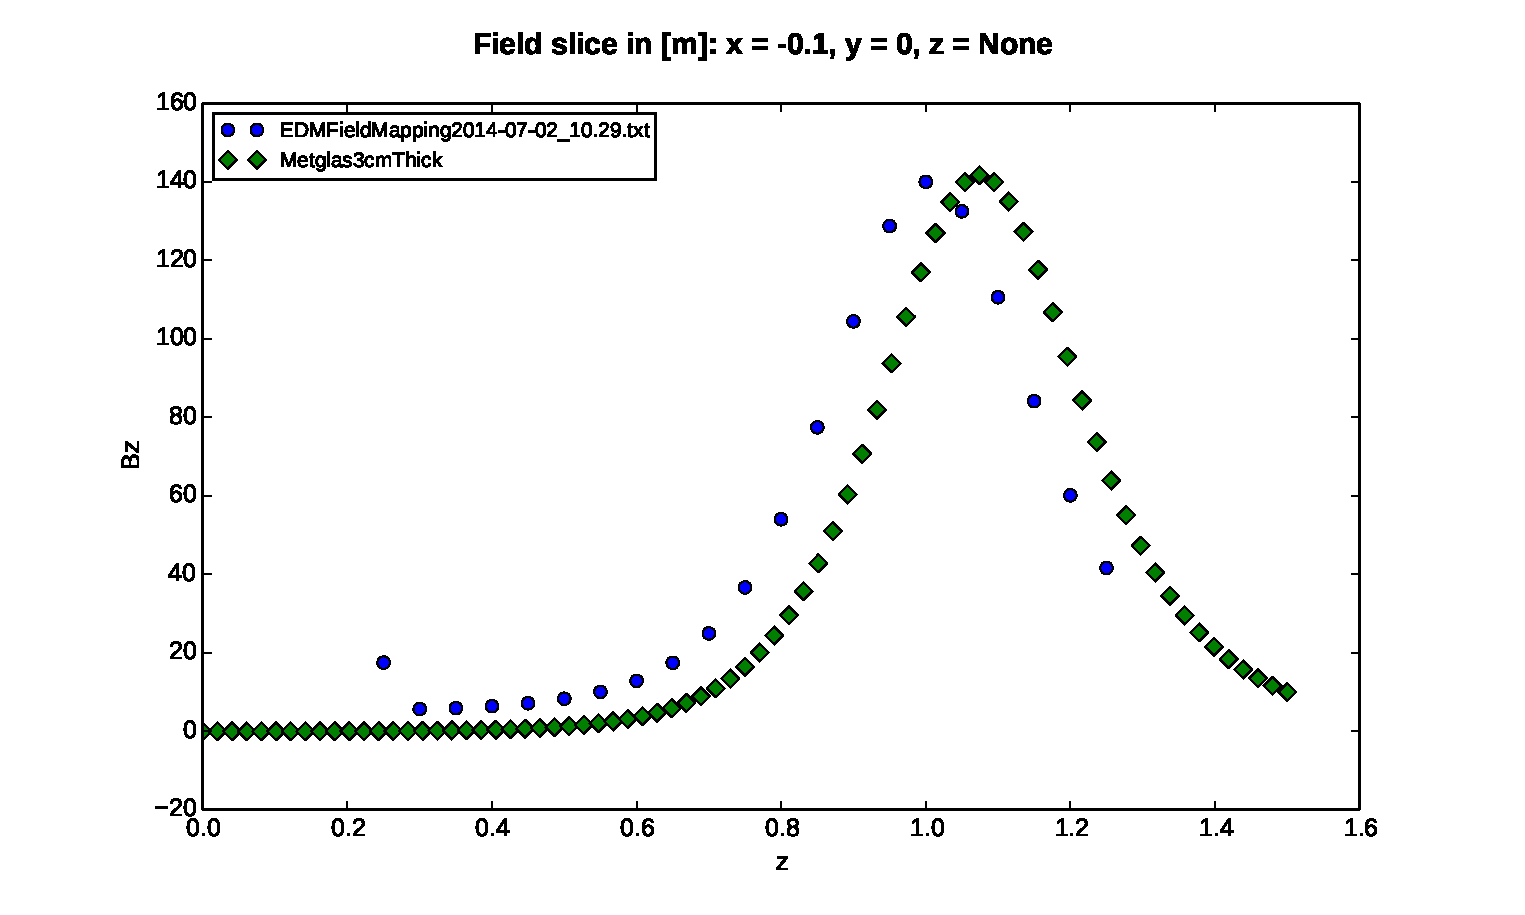
\includegraphics[width=0.95\textwidth]{../savedplots/original_Bz.eps}
\caption{\label{fig:orig_Bz_z}The magnetic field component $B_z$ [mG] vs. $z$ [m] along the line
$x = -0.1 \text{ m}, y = 0$. Green points are predicted by the \texttt{RotationShield} simulation, and blue points
are from the initial measured field map. The measurement shows the $B_z$ maximum occurring 10 cm lower than it should.}
\end{figure*}

\subsection{Cooldown}

During this time, we have also been cooling the lead shield and endcap. Once the lead temperature drops below
7 K, I will be able to take the first field map that includes a superconducting top endcap. By that point, I will
also have run high-resolution simulations that include the lead shield and top endcap. In the final weeks of SURF,
I will analyze that data and determine whether our endcap simulations are accurate and how effective the top endcap
will be for the final nEDM experiment.


\begin{thebibliography}{}
\bibitem{cpv} Cronin, J. ``Nobel Lecture: CP Symmetry Violation – The Search
for Its Origin,'' Nobel Media AB (2013).
\bibitem{ill} Baker, C. A., D. D. Doyle, P. Geltenbort, K. Green, M. G. D. Van der Grinten, P. G. Harris, P. Iaydjiev et al. ``Improved experimental limit on the electric dipole moment of the neutron.'' \textit{Physical Review Letters} 97, no. 13 (2006): 131801.
\bibitem{krl} ``Search for the nEDM at Caltech.'' Kellogg Radiation Laboratory
$\langle$krl.caltech.edu$\rangle$ (2014).
\bibitem{endcapstyles} Malkowski, S., R. Y. Adhikari, J. Boissevain, C. Daurer, B. W. Filippone, B. Hona, B. Plaster, D. Woods, and H. Yan. ``Overlap Technique for End-Cap Seals on Cylindrical Magnetic Shields.'' \textit{IEEE Transactions on Magnetics} 49, no. 1 (2013): 651-653.
\bibitem{coil} Perez Galvan, A., B. Plaster, J. Boissevain, R. Carr, B. W. Filippone, M. P. Mendenhall, R. Schmid, R. Alarcon, and S. Balascuta. ``High uniformity magnetic coil for search of neutron electric dipole moment.'' \textit{Nuclear Instruments and Methods in Physics Research Section A: Accelerators, Spectrometers, Detectors and Associated Equipment} 660, no. 1 (2011): 147-153.
\bibitem{rotshield} Mendenhall, M. P. \texttt{RotationShield} source. $\langle$https://github.com/mpmendenhall/rotationshield$\rangle$ (2014).
\end{thebibliography}

\end{document}
